\documentclass{article}

\usepackage[T1]{fontenc}
\usepackage[utf8]{inputenc}
\usepackage[italian]{babel}
\usepackage{graphicx}
\usepackage{float}

\title{ISO/IEEE 11073-10206 - ACOM (Abstract Content Information Model)}
\author{Riccardo Cambianica}
\begin{document}
    \maketitle
    \newpage
    \tableofcontents\newpage
    \section{ACOM Observation class}
        ACOM Observation class (da qui in poi chiamata semplicemente "la classe") descrive un modello generico per esprimere \textbf{osservazioni} fatte dai PHD. E' basato sull'oggetto metrico descritto dallo standard ISO/IEEE 11073-20601 e condivide molti attributi della risorsa analoga osservazione presente nello standard HL7 FHIR.
        \begin{figure}[H]
            \centering
            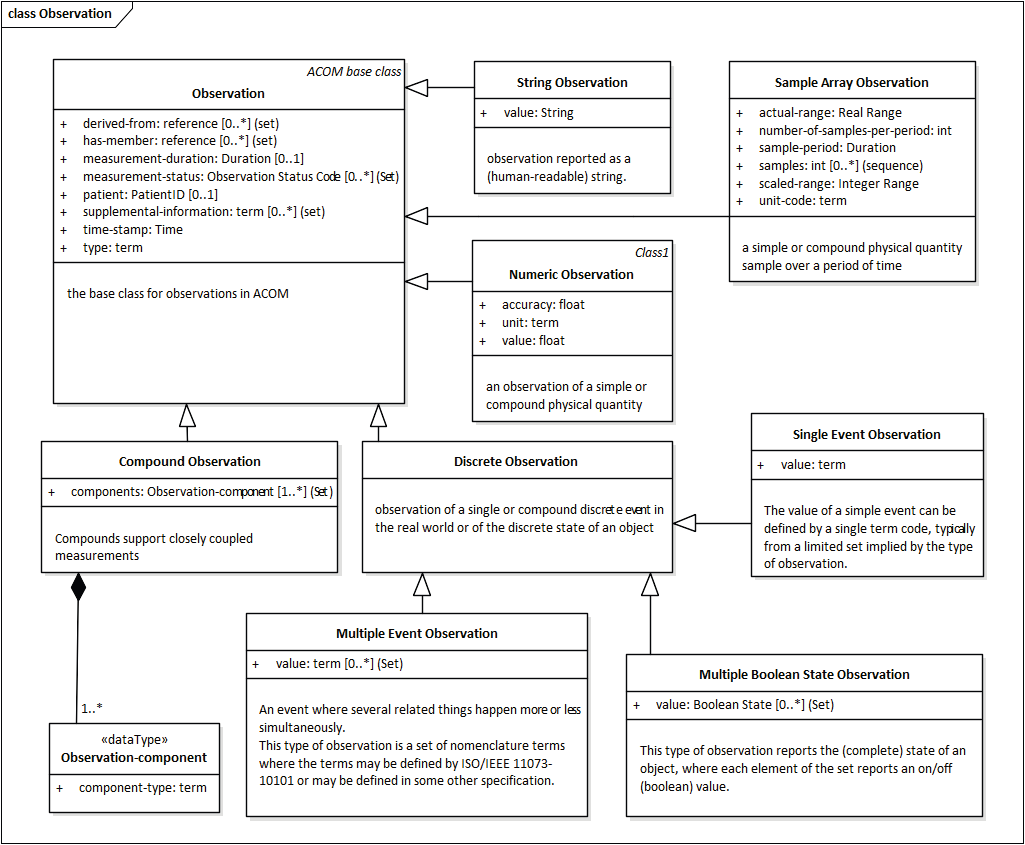
\includegraphics[width=1\textwidth]{figures/observation class.png}
            \caption{Classi in relazione con Osservazione}
            \label{fig:observationClass}
        \end{figure}
        Come si può vedere in figura \ref{fig:observationClass}, la classe si compone di alcuni attributi fondamentali: 
        \begin{itemize}
            \item prova 
        \end{itemize}
\end{document}